
\subsection{Rationale} \aanote{I think that the names of the states should be
removed. They are meaningless without the figures. I left them just in case we
decide to reintroduce the figures.}\mtnote{Done.} As seen in
\S\ref{sec:panda_deployment}, the absence of wide area network connectivity on
Titan's worker nodes was one of the main reasons for PanDA Broker not to
implement pilots. As discussed in \S\ref{sec:panda_titan}, the absence of pilots
imposes the static coupling between MPI scripts submitted to the PBS batch
system and detector simulations, and development tailored to each type of
payload that needs to be executed.

This static coupling makes impossible to schedule multiple generations of
workload on the same PBS job. Specifically, once a number of detector
simulations are packaged into a PBS job and this job is queued on Titan, no
further simulations can be added to that job. New simulations have to be
packaged into a new PBS job that needs to be submitted to Titan on the base of
the backfill availability of that moment.

The support of workload generations would enable a more efficient use of the
backfill availability of walltime. Currently, when a set of simulations ends
also the PBS job ends, independently on whether more walltime would still be
available. With a pilot, more simulations could be executed so to utilize all
the available walltime, while avoiding further job packaging and submission
overheads.

% \mtnote{Are there more reasons for wanting multiple generations?}

Multiple generations would also help with relaxing two assumptions of the
current execution model: knowing the number of simulations before submitting the
MPI script, having a fixed amount of events per simulation (100 at the moment).
Pilots would enable the scheduling of simulations independently from whether
they were available at the moment of submitting the pilot. Further, simulations
with a varying number of events could be scheduled on a pilot, depending on the
amount of remaining walltime and the distribution of execution time per event,
as shown in \S\ref{ssec:panda_titan}, Figure~\ref{fig:100event-distrib}. This
capabilities would be particularly useful to increase the PanDA Broker
efficiency for availabilities with a wide delta between the number of cores and
walltime.

% to one in which the number of events is decided on the base of the available
% walltime. Pilots would enable to package simulations with a heterogeneous
% number of events, especially when a small amount of cores is available for a
% long period of time and \textit{vice versa}. In these situations, a PBS job
% would require all simulations to have a small number of events that would not
% use all the available walltime.

% a pilot would instead support multiple generations of simulations with a
% different number of events and therefore duration.

Pilots can offer a payload-independent scheduling interface while hiding the
mechanics of coordination and communication among multiple worker nodes. This
could eliminate the need for packaging payload into MPI scripts within the
broker, greatly simplifying the submission process. This simplification would
also enable the submission of different types of payload, without having to
develop a specific PBS script for each payload. The submission process would
also be MPI-independent, as MPI is used for coordination among multiple worker
nodes, not by the payload.

% \mtnote{I tried to argue that pilots facilitates the submission to a normal
% queue but I was not able to find a convincing argumentation. When we consider
% only Titan, a PBS job is the only way to submit a job to its queue(s). With %
% NGE, we translate a pilot description to a PBS job and then submit it to a
% queue via a PBS command. PanDA Brokers do something very similar: they
% package detector simulations into a PBS job and they submit it via a PBS
% command. The fact that PanDA Brokers define the number of cores and walltime
% of a PBS job on the base of backfill information, does not make the packaging
% or the submission processes any different: PanDA Brokers are already
% submitting to the nomal queue. If I got it right, PanDA Brokers could already
% submit a job with, say, 12000 cores and 2 hours walltime. They don't do it
% because they have no allocation and they would wait a long time in the queue
% (maybe, let's see what our experiments say about that). I do not see how NGE
% could make all this any different.}

\mtnote{NOTE: I would speak about about backfill/not backfill in the discussion
of NGE, when speaking about its generality towards resources, i.e., unified
submission and scheduling process across different resources and multiple
resources. Part of this generality is being able to submit to whatever batch
system is supported by SAGA (including Titan's PBS and all its queues) and, in
case, to multiple resources at the same time.}

\mtnote{NOTE: NGE is not able to use backfill on Titan as we do not have
specific functionalities to interrogate the Moab scheduler about backfill
availability. This is why NGE should be presented as the pilot for PanDA Broker
and not as an alternative to PanDA Broker. Further, NGE alone would not be able
to speak directly to PanDA Server.}


% -----------------------------------------------------------------------------
\subsection{Architecture}
\label{sec:arch}

The implementation of pilot capabilities within the current PanDA Broker require
quantification of the effective benefits that it could yield and, on the base of
this analysis, a dedicated engineering effort. We developed a prototype of a
pilot system capable of executing on Titan to study experimentally the
quantitative and qualitative benefits that it could bring to PanDA. We called
this prototype Next Generation Executor (NGE).

% We developed and we are currently integrating a prototype of Next Generation
% Executor (NGE) to add pilot capabilities to the PanDA Broker.

NGE is a runtime system designed to execute heterogeneous and dynamic workloads
on diverse resources. Fig.~\ref{fig:arch-overview} illustrates its current
architecture as deployed on Titan: the two management modules represent a
simplified version of the PanDA Broker while the agent module is the pilot
submitted to Titan and executed on its worker nodes. The communication between
PanDA Broker and PanDA Server is abstracted away as not immediately useful to
evaluate the performance and capabilities of a pilot on Titan.

% Thus, workloads and pilots are described via the Pilot API and passed to the
% NGE runtime system. NGE launches the pilots and executes the tasks of the
% workload on them.

\begin{figure}
  \centering
   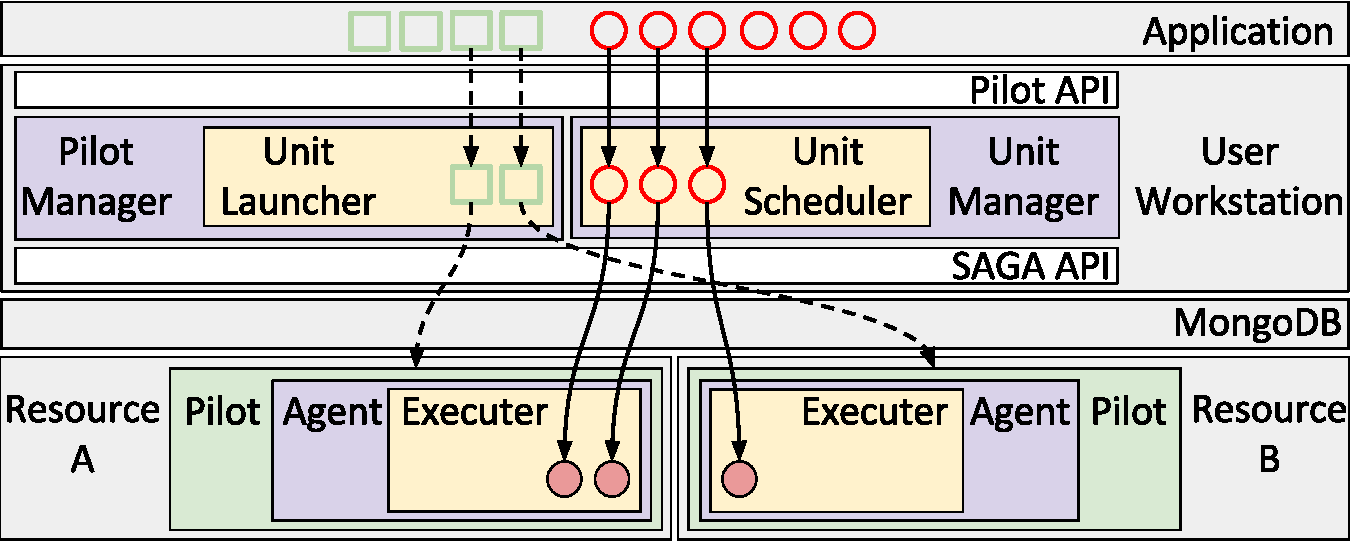
\includegraphics[width=\columnwidth]{figures/architecture_compact_rp_paper.pdf}
  % \caption{RP overview. An application uses the Pilot API to describe pilots
  %   (green squares) and units (red circles). The PilotManager (purple box)
  %   instantiates (dash arrow) pilots, the UnitManager (purple box)
  %   instantiates (solid arrow) units. Both managers are executed on the user
  %   workstation. Pilots are launched (dashed arrows) on resources A and B
  %   via SAGA API, an Agent (purple box) is bootstrapped for each pilot
  %   (green box), units (solid red circles) are scheduled to the Agents via
  %   MongoDB and executed by the Agent's Executer (yellow box).
  \caption{NGE Architecture as deployed on Titan. The PilotManager and the
  UnitManager reside on one of Titan's DTN while the Agent is executed on
  Titan's worker nodes. Boxes color coding: gray for entities external to NGE,
  white for APIs, purple for NGE's modules, green for pilots, yellow for
  module's components.\mtnote{Change the picture eliminating Resource B.}}
\label{fig:arch-overview}
\end{figure}

% Internally, NGE represents pilots as aggregates of resources independent from
% the architecture and topology of the target machines, and workloads as a set
% of units to be executed on the resources of the pilot. Both pilots and units
% are stateful entities, each with a well-defined state model and life cycle.
% Their states and state transitions are managed via the three modules of the
% NGE architecture: PilotManager, UnitManager, and Agent
% (Fig.~\ref{fig:arch-overview}, purple boxes).


NGE exposes an API for the application layer to describe workloads
(Fig.~\ref{fig:arch-overview}, green squares) and pilots
(Fig.~\ref{fig:arch-overview}, red circles), and to instantiate a PilotManager
and a UnitManager. The PilotManager submits (Fig.~\ref{fig:arch-overview}, dash
arrow) pilots to Titan's PBS batch system via SAGA API, as done by PanDA Broker
to submit MPI scripts. Once scheduled, the pilot's Agent is bootstrapped on
Titan's workers nodes, and  the UnitManager schedules
(Fig.~\ref{fig:arch-overview}, solid arrow) units to the Agent's Executer for
execution. The UnitManager and the Agent communicate via a database that is
instantiated on one of Titan's DTN so to be reachable by both modules. A similar
approach would be used to enable PanDA Broker to schedule pilots instead of MPI
scripts.

% The lifespan of pilots has four states distributed among the PilotManager,
% resource, and pilot instance.% (Fig.~\ref{fig:pilot-state-model}).
% Pilots are instantiated in the state \T{NEW} by the PilotManager, wait in a
% queue to be launched, and transition to \T{PM\_LAUNCH} when submitted to a
% Resource Manager (RM) via the SAGA API\@. Pilots wait in the queue of the RM
% and, once scheduled, become \T{P\_ACTIVE}. They remain in this state until the
% end of their lifetime, when they transition to \T{DONE}.

%\begin{figure}
%  \centering
%  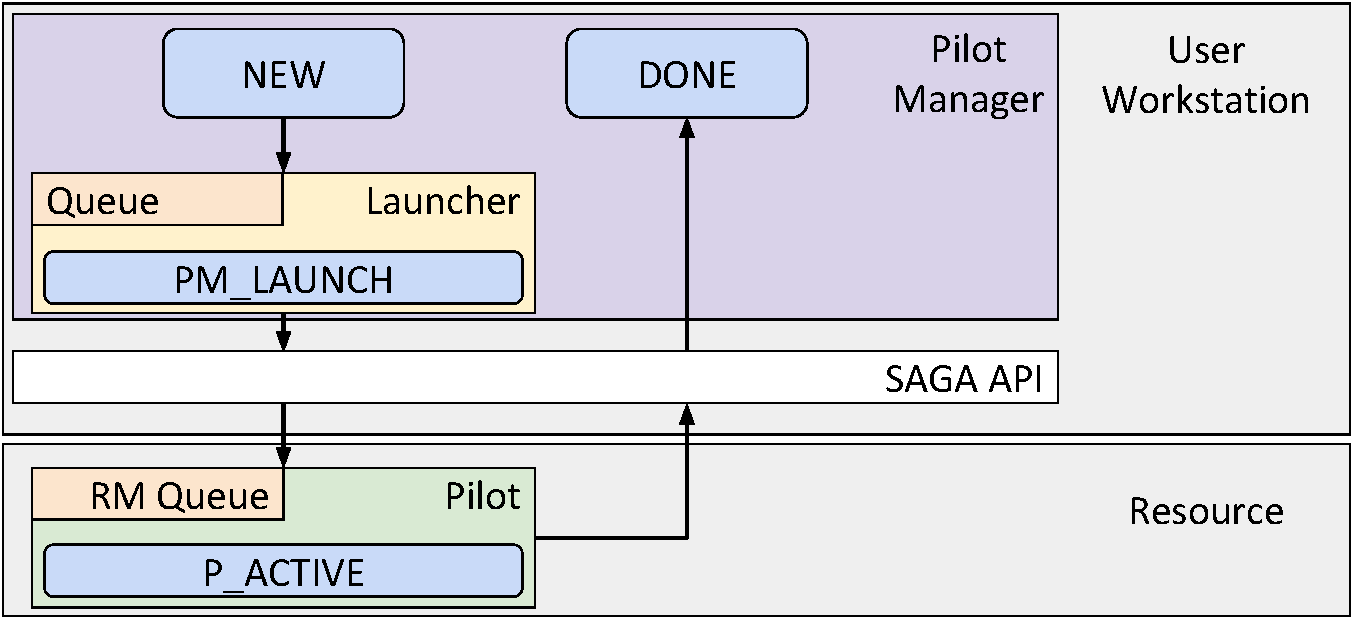
\includegraphics[width=\columnwidth]{figures/pilot_state_model_compact_rp_paper.pdf}
%  \caption{Pilot State Model. Instantiated in state \T{NEW}, each pilot is
%    launched (\T{PM\_LAUNCH}) via SAGA API on a resource manager. After
%    becoming \T{P\_ACTIVE}, it exhausts its duration ending in state
%    \T{DONE}. The transition between states is sequential and each transition
%    can be canceled or fail ending in the states \T{CANCELED} or \T{FAILED} (not
%    depicted to improve the diagram clarity). Boxes color coding as per
%    Fig.~\ref{fig:arch-overview}, with: orange for queues and blue for states.
%\label{fig:pilot-state-model}}
%\end{figure}
%

% The unit state model has nine states distributed across the UnitManager,
% MongoDB instance, and Agent.% (Fig.~\ref{fig:unit-state-model}).
% Instantiated in the state \T{NEW} by the UnitManager, every unit is scheduled
% on an Agent (\T{UM\_SCHEDULING}) via a queue on a MongoDB instance. The unit
% is then scheduled on the required number of cores held by the Agent's pilot
% (\T{A\_SCHEDULING}), and finally executed (\T{A\_EXECUTING}).

% The unit state model pertains also to the input and output data of the units.
% When required, the input data of a unit are either pushed to the Agent
% (\T{U\_STAGING\_IN}) or pulled from the Agent (\T{A\_STAGING\_IN}), depending
% on data locality and sharing requirements. Similarly, the output data of the
% unit are staged out by the Agent and UnitManager (\T{A\_STAGING\_OUT},
% \T{U\_STAGING\_OUT}) to a specified destination, e.g., the user workstation.
% Both input and output staging are optional, depending on the requirements of
% the units. The actual file transfers are enacted via SAGA, and support
% (gsi)-scp, (gsi)-sftp, and Globus Online.

%\begin{figure}
%  \centering
%  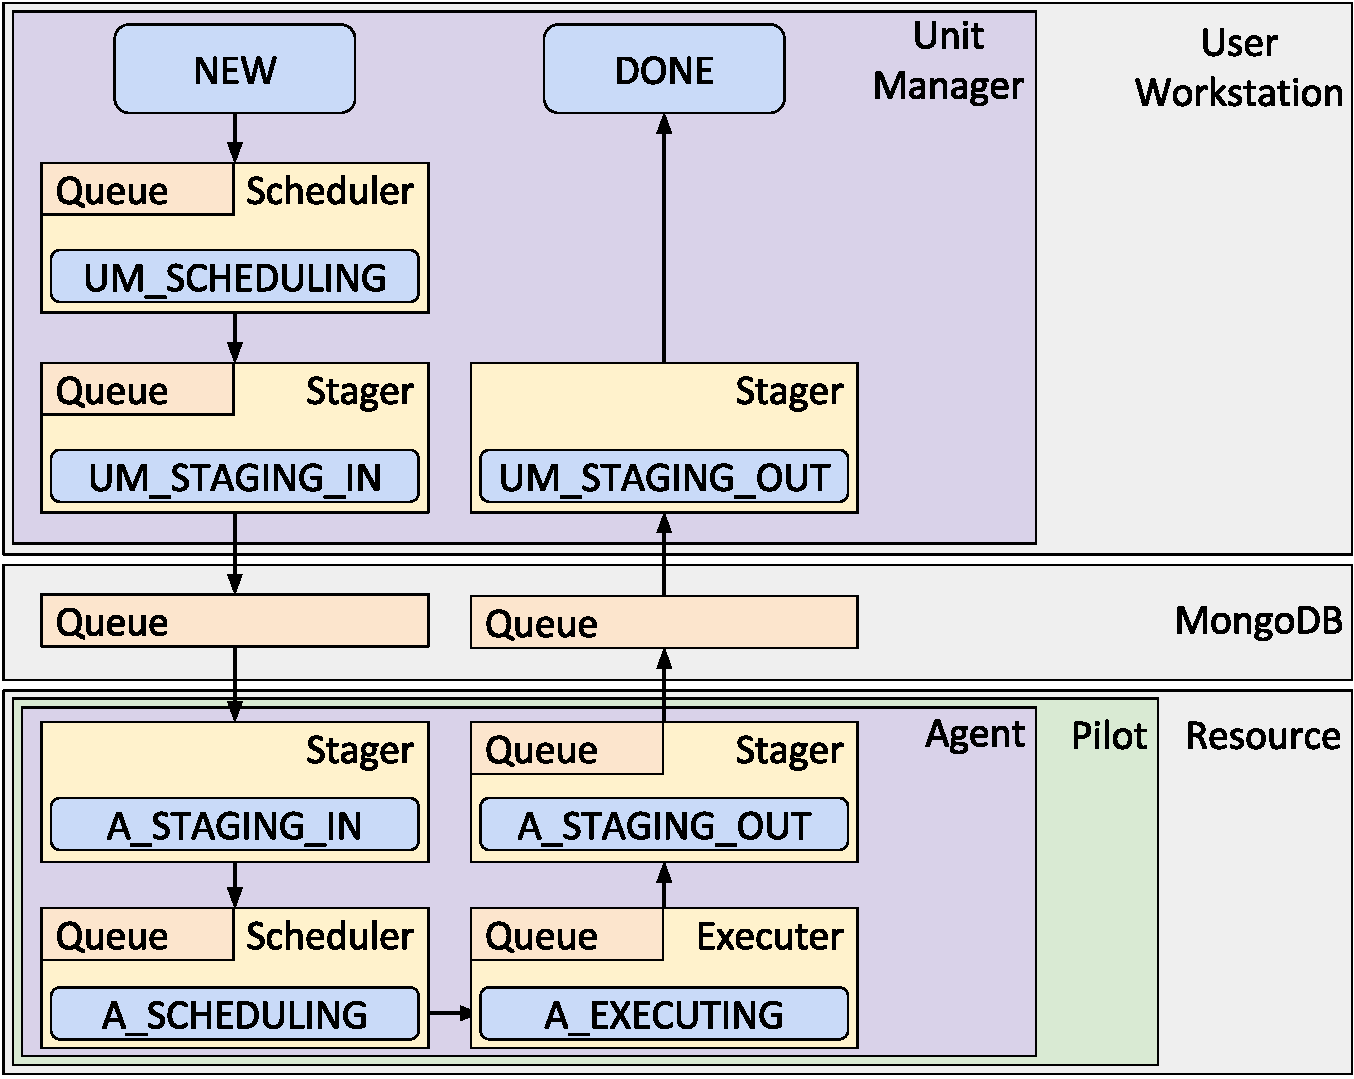
\includegraphics[width=\columnwidth]{figures/unit_state_model_compact_rp_paper.pdf}
%  \caption{Unit State Model. Instantiated in state \T{NEW}, each unit is
%    scheduled to an Agent (\T{UM\_SCHEDULING}) via MongoDB, and then scheduled
%    to an Agent's Executer (\T{A\_SCHEDULING}). When required, unit input data
%    are staged to the Agent's Pilot (\T{UM\_STAGING\_IN} or
%    \T{A\_STAGING\_IN}). Each unit is executed (\T{A\_EXECUTING}), unit output
%    data are staged out (\T{A\_STAGING\_OUT} and \T{UM\_STAGING\_OUT}), and
%    each unit ends in state (\T{DONE}). Color coding and state omissions
%    as per Fig.~\ref{fig:pilot-state-model}.
%\label{fig:unit-state-model}}
%\end{figure}

%The state transitions represented in Figures~\ref{fig:pilot-state-model}
%and~\ref{fig:unit-state-model} are sequential and every transition can fail or
%be canceled by the PilotManager or UnitManager.

% All state transitions are managed by the PilotManager, UnitManager, and Agent
% components. The only special case is the transition of the pilots to the state
% \T{P\_ACTIVE} which is dictated by the resource's RM, but managed by the
% PilotManager.

% Above all NGE's components, the Agent is the one that is worth to mention the
% most.

Agents of NGE run on MOM nodes or worker nodes, using the \emph{Open Run-Time
Environment (ORTE)}. ORTE is a spin-off from the Open-MPI project and is a
critical component of the OpenMPI implementation. It was developed to support
distributed high-performance computing applications operating in a heterogeneous
environment. The system transparently provides support for interprocess
communication, resource discovery and allocation, and process launching across a
variety of platforms. ORTE provides a mechanism similar to the Pilot concept -
it allows the user to create a \emph{``dynamic virtual machine''} (DVM) that
spans multiple nodes. ORTE provides libraries to enable the submission,
monitoring and managing of tasks, avoiding filesystem bottlenecks and race
conditions with network sockets. As a consequence, it is able to minimize the
system overhead while submitting tasks.

%Each component of RP has a independent semantic scope. This enables modularity
%isolating implementation complexity and supporting diverse use cases and
%environments.  For example, unit scheduling can be implemented by exchangeable
%Scheduler components, suitable for applications of diverse scales, with
%different coordination patterns, and executed on Beowulf clusters or Cray
%machines.
%
%Components are also designed to be stateless and instantiated concurrently. In
%this way, RP can manage multiple pilots and units at the same time, resulting
%in scalable throughput and tolerance to failing components. Concurrent
%components are coordinated via a dedicated communication mesh which incurs
%infrastructure and runtime overhead, offset by the lower component complexity
%and improved overall scalability of the system.

% \begin{enumerate}
%     \item Rationale and design (why)
%     \item Architecture (how)
%     \item Integration (Not present)
%     \item Characterization (experiments)
% \end{enumerate}

 % \ldots
